\documentclass[portfolio.tex]{subfiles}

\begin{document}
	\Chapter{Week 3}{JavaScript In Depth}
		\label{week-3-js}
		\section{Introduction}
			This week extends our knowledge on JavaScript from week 1 (\ref{week-1-js}), by introducing control statements, arrays, operations, JSON and jQuery. These concepts allow us to do more than simply modify the DOM and begin to incorporate logic into the websites.

		\section{Weekly Content}
			\subsubsection{Control Statements}
				Control statements allow us to create different paths that can be traversed in programs depending on certain conditions. \\

				\textbf{If} statements check a boolean expression (something is either true or false) and if the result of that expression is true, the actions within that block will be executed. There is also an \textbf{else if} statement that can occur directly after an if statement. This statement only occurs if the if statement was false, and the supplied boolean expression is true. The last piece of this chain is an \textbf{else} statement. If all previous if and else if statements were false, the code within the else block will execute.  \\

				\begin{lstlisting}
If(x > 0) {
	return "x is a positive number";
} else if (x < 0) {
	return " x is a negative number";
} else {
	return "x is 0";
}
				\end{lstlisting}

				\vspace{0.5cm}

				\begin{center}
					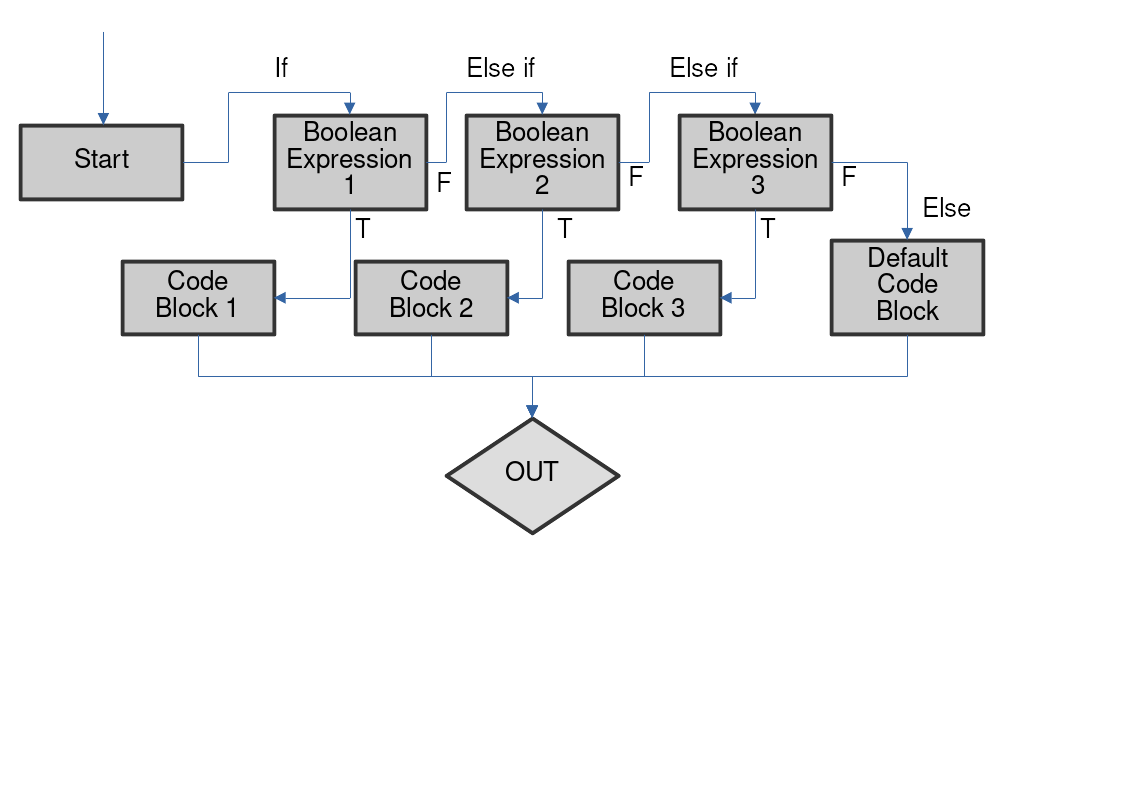
\includegraphics[trim=0 250 0 0, clip, width=0.8\textwidth]{Control Statements.png}
				\end{center}


				For statements that have many options, a \textbf{switch} statement would be a better option. In a switch statement, the interpreter will compare the variable against each value. Once a value matches the variable, the remaining code will be executed, or until a \textbf{break} is reached. A good code practice should be to always have a default case that runs if none of the other cases match. Here is an example of a switch statement from the lecture that I have modified:\\

				\begin{lstlisting}
switch(fruit) {
	case 'Oranges':
		console.log('$0.59 a pound.');
		break;
	case 'Mangoes':
		console.log('$2.49 a pound.');
	case 'Papayas':
		console.log('$2.79 a pound.');
		break;
	default:
		console.log('Sorry, we are out of these');
}
				\end{lstlisting}

				\vspace{0.5cm}

				This demonstrates the importance of remembering the break. In this code if the fruit was Mangoes, Both the \$2.49 a pound, and the \$2.79 a pound messages would print. There might be cases when you would want multiple variables to perform the same action. In this case omitting the break is necessary. \\

				\textbf{Try/catch} blocks is another control statement. Code within the try block is executed as normal, and if an error occurs, the code within \textbf{catch} block will run. This allows the program to handle the error smoothly. To highlight the importance of the try/catch; if an error occurred outside of a try block, the program would immediately stop (\textbf{crash}) and display an error code. In the following example, we are able to log a message to the console, and then proceed to ask the user for a new file name. \\

				\begin{lstlisting}
try {
	file = readFromDisk();
} catch (error) {
	console.log("File was not found")
	askUserForNewFile();
}
				\end{lstlisting}

			\subsection{Arrays}
				Arrays are a collection of values stored in one variable in contiguous memory. Elements of an array can be accessed by their index (which starts at 0 in JavaScript). The syntax in JavaScript is to use square brackets, for example: \textit{array[2]} would give the third value  of the array. \\

				\begin{center}
					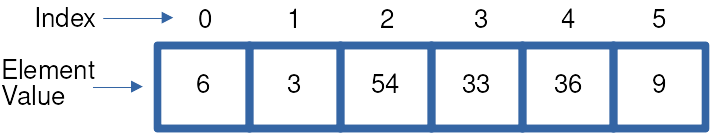
\includegraphics[trim=0 550 350 100, clip, width=0.8\textwidth]{Array.png}
				\end{center}

			\subsection{JSON}
				JSON is a format for storing data. It uses key-value pairs to describe the data, the same way that objects are created in JavaScript, hence the name JavaScript Object Notation. Basic data structures can also be nested inside keys using the curly brackets \{\} for an object, or square brackets [] for an array. \\

				\begin{lstlisting}
{
	"name":"John",
	"age":31,
	"children" :["Sarah","Harry"],
	"contact":{
		"phone":123-232-2323,
		"email":"john@john.com"
	}
}
				\end{lstlisting}

			\subsection{Operators}
				Operators allow us to compare two expressions. Here are some of the operators within JavaScript:\\

				\begin{tabular}{|P{2cm}|p{14cm}|}
					\hline
					$>$&  Is true if the left value is greater than the right.\\
					\hline
					$<$&  Is true if the left value is less than the right.\\
					\hline
					==&  Is true if both values are equal.\\
					\hline
					!=&  Is true if both values are not equal.\\
					\hline
					\&\&&  Combines two logical statements, only true if both individual expressions are true.\\
					\hline
					$\|$&  Combines two logical statements, true if either expression are true (or both).\\
					\hline
					\& &  Applies a bitwise AND to each value. That is goes bit by bit, through both variables and returns 1 if they are both 1, otherwise it returns the zero. The results are stored in a third variable. For example 10011 \& 11001 = 10001. \\
					\hline
					\textbar &   The same as \&, but it applies a bitwise OR. Returns 1 if either bit is one, but returns 0 if both are the same.\\
					\hline
					\^{} &  The same as | but will also return 1 if both bits are 1. (Bitwise XOR)\\
					\hline
					===\newline !== & The difference between === and == is that === also checks type. For example 0 == "0" is true, but 0 === "0" is false.\\
					\hline
				\end{tabular}

			\subsection{jQuery}
				jQuery is a framework that shortens the amount of code needed when performing common JavaScript tasks. For example, instead of:\\
				 \begin{center}
					\textbf{document.getElementById("id").hide();}\\
				 \end{center}
				jQuery allows a shorter command:

				\begin{center}
					\textbf{\$('\#id').hide();}
				\end{center}
				 The \$ is shorthand to show that it is a jQuery command. \\

				Another area where jQuery helps reduce the amount of code is in network calls using AJAX. AJAX is \textbf{A}synchronous\textbf{ J}avascript \textbf{A}nd\textbf{ X}ml. This allows to create calls to external urls, and then call function based on success or failure. This allows easy manipulation of the DOM based on queries to backend servers.

		\section{Practical Tasks}

			JavaScript has many built-in libraries and class methods. These accomplish common tasks, so developers don't have to constantly "re-invent the wheel". \\

			\noindent These tasks help reinforce being able to learn and understand the documentation. This is critical when working on web applications since you won't always have an instructor to run to when things go wrong, and must learn to teach yourself.

			\subsection{Task 1}
				 Task 1 was all about string manipulation. Since websites are about displaying information, manipulating strings occurs often. Since strings are objects in JavaScript, they come with some built-in methods. Some common methods are:\\

				 \begin{tabular}{|P{4cm}|p{10cm}|}
				 	\hline
				 	string.length & Returns the number of characters in a string. \\
				 	\hline
				 	\hspace{0.3cm}string.splice() \newline string.slice() & Two very similar methods. They return the characters between the specified start index and end index. The difference is that splice removes the character from the original string, while slice leaves the original string intact. \\
				 	\hline
				 	string.replace()& Finds the first argument within the string, and replaces it in the second argument. The first argument can also be a \textbf{Regular Expression}, making this function very powerful. \\
				 	\hline
				 	string.toLowerCase() \newline string.toUpperCase() & Turns every character either lowercase or uppercase respectively. \\
				 	\hline
				 	string.trim() & Removes any extra white-space at the beginning and the end of the string.  \\
				 	\hline
				 	\hspace{0.3cm}string.padStart() \newline string.padEnd() & Ensures the string is a certain length by adding padding if necessary. padStart() adds the specified padding character to the beginning, and padEnd() adds the padding to the end. \\
				 	\hline
				 \end{tabular}

			 	\autocite{string-methods}\\

			 	\subsubsection{Screenshot}
			 	\begin{center}
				 	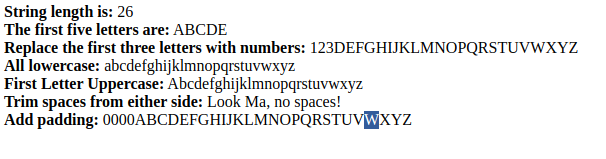
\includegraphics[width=8cm]{Prac-3-Task-1.png}
			 	\end{center}


			 	\subsubsection{Source Code}
				The source code for my task can be found at \seqsplit{https://github.com/BrandonMurch/SIT120/blob/021a2694432d61e32c9fba191ee7579c2dfdb955/Practical\%20Tasks/Practical\%203/Task1.html}


			\subsection{Task 2}
				The second task involved using Number methods and Array methods. These methods are similar to the idea of the methods in task 1, but they apply to numbers and arrays respectively.\\

				\subsubsection{Number methods}

				\hspace{-0.5cm}
				\begin{tabular}{|P{0.33\linewidth}|p{0.66\linewidth}|}
					\hline
					number.toString() & Changes the number to the type "string".  \\
					\hline
					number.toExponential() & Returns the number in exponential form. \\
					\hline
					number.toFixed() & Returns the number, with a fixed amount of decimal places. \\
					\hline
					number.toPrecision() &  Returns the number with a fixed number of digits. \\
					\hline
					parseInt() & Takes a string and returns it as a Number if possible.   \\
					\hline
					Math.round() \newline Math.ciel() \newline Math.floor() &  Round the number to the nearest digit. ciel always rounds up, floor always round down. \\
					\hline
					Math.random() & Gives a random number between 0 and 1. \\
					\hline
				\end{tabular}
				\autocite{number-methods}\\

				\subsubsection{Array methods}
				\begin{tabular}{|P{4cm}|p{12cm}|}
					\hline
					array.toString() & Converts the array to a string. \\
					\hline
					array.join() & Same as toString, but can specify what characters to place in between elements.  \\
					\hline
					Array.from() & Returns a new array from whatever is provided as an argument. Useful for duplicating arrays.  \\
					\hline
					array.pop()  \newline array.shift() & Removes and returns the last or first element of the array respectively.  \\
					\hline
					array.push() \newline array.unshift() & Adds a value to the end or beginning of the array respectively. Returns the array length. \\
					\hline
					array.concat() &  Merges an array passed as an argument into the original array.  \\
					\hline
				\end{tabular}
				\autocite{array-methods}\\

				\subsubsection{Screenshot}
				\begin{center}
				 	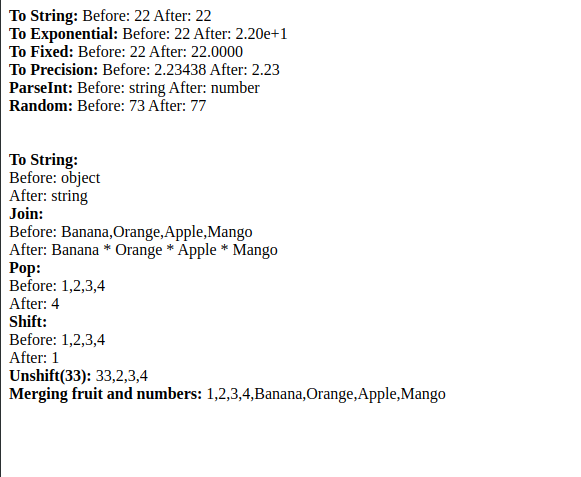
\includegraphics[trim=5 20 0 0, clip, width=8cm]{Prac-3-Task-2.png}
				\end{center}


			 	\subsubsection{Source Code}
				The source code for my task can be found at \seqsplit{https://github.com/BrandonMurch/SIT120/blob/021a2694432d61e32c9fba191ee7579c2dfdb955/Practical\%20Tasks/Practical\%203/Task\%202.html}.

			\subsection{Task 3}
				JavaScript objects have methods for getting and setting internal values. This is an example of encapsulation, a main concept of object-oriented design. Instead of having access to the variables directly, the objects are interacted with using GET functions and SET functions. GET functions return the value of the variable. SET functions take the new value as an argument, and then changes the value of the variable internally. \\

				Date is an object built into JavaScript that stores a particular date and time. This uses get functions to get either the whole date formatted in a particular manner, or parts of the date such as hours, months, etc. The set function of the date object allows the caller to set a particular part of the date such as hours, months, etc.

				\subsubsection{Screenshot}
			 	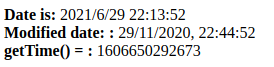
\includegraphics[width=4cm]{Prac-3-Task-3.png}

				\subsubsection{Source Code}
				The source code for my task can be found at \seqsplit{https://github.com/BrandonMurch/SIT120/blob/021a2694432d61e32c9fba191ee7579c2dfdb955/Practica\%20Tasks/Practical\%203/Task\%203.html}.

			\subsection{Task 4}
				\subsubsection{Reflection}
					This task was all about looking ahead to the basic concepts of Vue. Understanding the concepts well will allow us to more easily implement these concepts in code.

				\subsubsection{Computed Property}
					Computed property is a property based on another property. It is a function that modifies another property and returns a value. This reduces the redundancy of code by reusing these functions instead of putting them directly in the template.  Another benefit to using computed properties is that they are cached for better performance, and is only re-called when the original property is modified.\\

					\hspace{-0.5cm}Computed Properties are assigned using the \textbf{computed} key inside the component object. \autocite{vue-computed}

				\subsubsection{Watcher}
					Watchers are a more generic version of computer property. The two are different because Watchers allow the observation of external variables and are not restricted to Vue Properties. This is useful when using asynchronous calls as the base data. \\

					\hspace{-0.5cm}Watchers are assigned using the \textbf{watch} key inside the component object. \autocite{vue-computed}
				\subsubsection{Class and Style Bindings}
					Vue allows classes to be dynamically assigned based on variables. An object is passed in to the attribute where the keys are the classes, and the paired values are the variables being evaluated. If the variable is truthy, then the class will be applied. Many classes can be put into the object.\\

					\hspace{-0.5cm}Styles can also be assigned dynamically by passing in an object with style key-value pairs.\\

					\hspace{-0.5cm}Class and Style bindings use the \textbf{v-bind:class=""} or \textbf{v-bind:style =""} syntax respectively. \autocite{vue-class}

				\subsubsection{Conditional Rendering}
					Conditional rendering allows the browser to render an element only a boolean expression is true. If true, then the element will be rendered. If not, the element will not be rendered.\\

					\noindent Conditional rendering uses the \textbf{v-if} attribute in the html or templates. This can be combined with \textbf{v-else-if and v-else} to create multiple outcomes. \autocite{vue-conditional}

				\subsubsection{List Rendering}
					List rendering renders a component or template using each element in a list as the passed in value. For example, if there was a list of [1,2,3], it would render one element, and pass in 1, render the same element again and pass in 2, then finally render element once more and pass in 3. This is very useful if you have a list of items that need to be rendered and reduces the code needed to accomplish this.\\

					\noindent This uses the \textbf{v-for} attribute in the html or templates. \autocite{vue-list}

				\subsubsection{Event Handling}
					This allows Vue to monitor for specified actions being performed on the element. For example \textbf{v-on:click} will run whatever function is given when the element is clicked. This also allows the direct modification of component data instead of a function (for example: v-on:click="counter += 1" would increment the counter on click). Methods can be written in directly, or placed in the methods object within the component. \autocite{vue-event}

				\subsubsection{Form Input Bindings}
					Form input bindings allow Vue to directly link inputs to variables. Whenever the value of an input changes, the variable in the component is updated. This is done by placing the variable being updated into the \textbf{v-model} attribute on the input element. \autocite{vue-list}
				\subsubsection{Component Basics}
					Components allow reusing templates, methods, etc. based on different values being passed in. This allows many of these components to be created without having to retype the boilerplate code, methods, etc. This also also provides easy consistency when it comes to style. \\

					A new component is defined in the JavaScript file. It gets created by calling \textbf{Vue.component()} and passing in the name of the component, as well as an object will all of the data, template, methods, etc.. \autocite{vue-component}


		\section{Project}
			\subsection{What I achieved this week}
				This week I have completed the remaining parts of my proposal. I designed every webpage in Figma, meaning the implementation should be quite painless. I have planned out the layout of my code and am ready to get started.

			\subsection{What I need to achieve next week}
				Next week I must start creating my webapp using HTML/CSS/JS/Vue. Specifically I would like to target the Nav bar and Image gallery components. This are probably the more complicated components within the web app and also the most reused. This should take me 4 hours.


\pagebreak
\end{document}